
\section{GAT-Denoiser}

\begin{frame}{GAT-Denoiser}
  \begin{itemize}
    \item GAT-Denoiser is a graph neural network (GNN) to denoise observations.
    \item Consists of three components:
    \begin{itemize}
      \item Convolution
      \item Graph Attention Network (GAT) \cite{GAT}
      \item End-to-End Learning
    \end{itemize}
  \end{itemize}

  \only<2>{
    \begin{figure}
      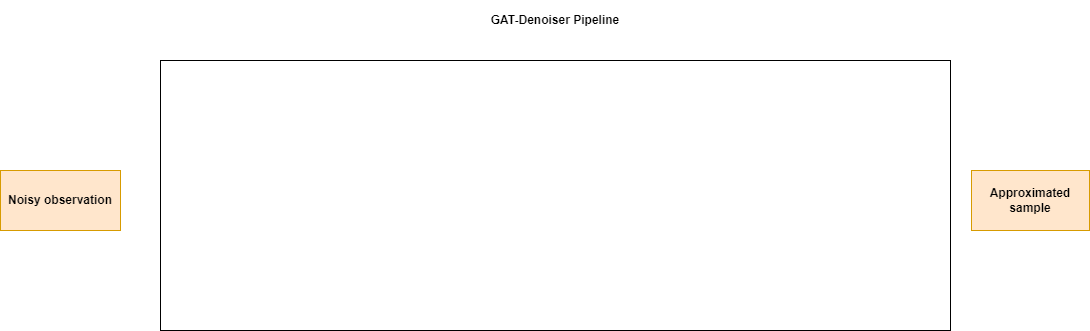
\includegraphics[width=\textwidth]{Overall_GAT-Denoiser_Pipeline_3.drawio.png}
    \end{figure}
  }

  \only<3>{
    \begin{figure}
      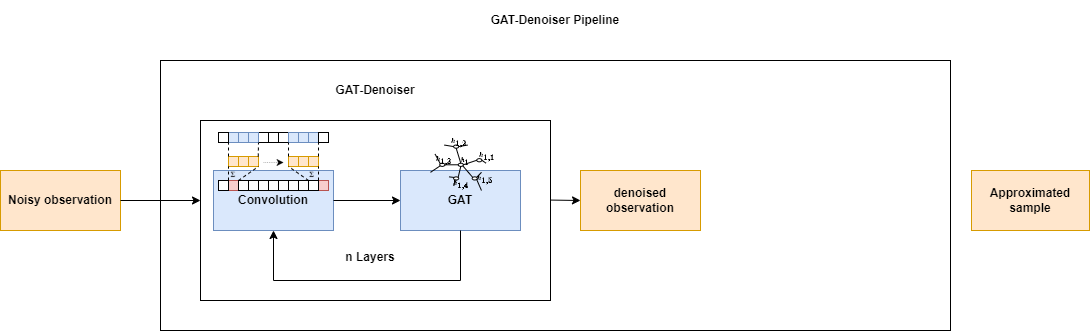
\includegraphics[width=\textwidth]{Overall_GAT-Denoiser_Pipeline_2.drawio.png}
    \end{figure}
  }

  \only<4>{
    \begin{figure}
      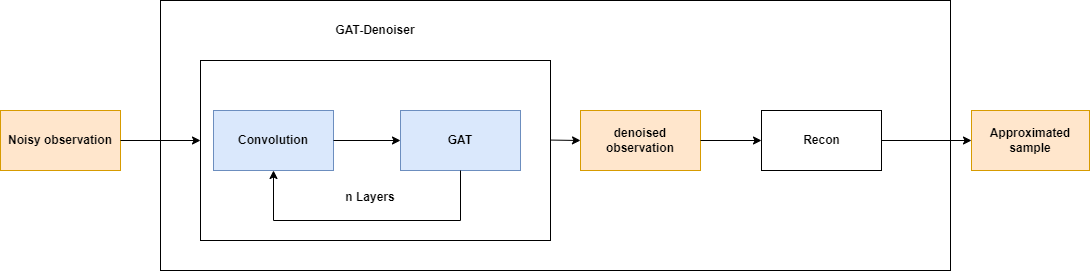
\includegraphics[width=\textwidth]{Overall_GAT-Denoiser_Pipeline.drawio.png}
    \end{figure}
  }

\end{frame}

\begin{frame}{Input Graph}
  \begin{columns}
    \column{0.5\textwidth}
    \begin{itemize}
      \item Exploit information for GL
      \item Low-dimensional embedding estimated angles
      \item Dominant information in data can be considered observation angles.
      \item Data will be processed on a circle graph.
    \end{itemize}
    \column{0.5\textwidth}
    
  \end{columns}
  

  \begin{tcolorbox}[colback=red!5!white,hide=<-1>, alert=<2>, colframe=red!75!black]
    Only single particle cryo-EM is considered.
\end{tcolorbox}


\end{frame}

\begin{frame}{Graph Attention Network - GAT}
  GAT, straight to the point
\end{frame}

\begin{frame}{Expectation from components}
  expections from convolution,   
\end{frame}

